\documentclass[]{article}
\usepackage[numbers]{natbib}
\usepackage{hyperref}
\hypersetup{colorlinks=true,allcolors=blue}
\usepackage{hypcap} 
\usepackage{graphicx}
\usepackage[margin=1.3in]{geometry}
\usepackage{musixtex}
\usepackage{listings}


\lstdefinestyle{mybashcode}{
  basicstyle=\linespread{0.8}\scriptsize\ttfamily,
  postbreak=\space,
  captionpos=b,
  aboveskip=15pt,
  abovecaptionskip=8pt,
  % belowcaptionskip=0pt
}

\graphicspath{ {Figures/} }

\makeatletter
\renewcommand\maketitle {
  \begin{center}
    {\Large{\course}}
    \medskip\par\noindent
    {\Large\textbf{\@title}}
    \medskip\par\noindent
    {\Large\@author}
    \medskip\par\noindent
    {\Large\@date}
    \bigskip\par\noindent
  \end{center}
}
\makeatother

\newcommand{\course}{CSCE 790-002: Deep Reinforcement Learning and Search}
\title{Musical Deep Reinforcement Learning}
\author{Francisco Vilchez}

\begin{document}

\maketitle

% Deep Reinforcement learning to music: \cite{deeprl2016music}
% Plain results, seems that it never changes key

% Google results (magenta): \cite{magenta2018}

% Connectionist old explanation: \cite{connectionist1989}

% RRN in music (blues): \cite{eck2002blues}
% Not good results. Sounds weird
% too many jumps
% seems that it is not fitting in the chord

% Evaluation is relative: \cite{biles2013lessons}

\section*{Abstract}
Computational musical composition tries to teach a computer what the best sequence of notes to play would be. This can become an interesting task, since there is no specific process to measure whether one composition will sound better than another one, therefore, its quality value depend on each person musical preferences. In this project, we proposed using Deep Reinforcement Learning to capture the feedback from users during training so that way the computer can learn based on what the user consider is a good melody. Our project confirmed that the musical composition problem can fit into a Reinforcement Learning problem. It was able to learn policies according to the feedback that it was given while it played its composition and store it in order to continue the learning process later. Results of the project are available in Github\footnote{Code available at: https://github.com/franciscovilchezv/eurydice.rl}.

\section*{Introduction}
In this project we will try to solve the automated musical composition problem using Reinforcement Learning and Recurrent Neural Networks. Musical composition is an interesting problem in Computer Science since it deals with a big difficulty which is trying to teach a computer how to evaluate if a composition sounds good, and maybe even more difficult situation, which is to compare to musical melodies and decide which of the has a better sound. Because of that, automated musical composition requires the usage of innovative methods that try to get close to the way humans (or musicians) take decisions. Additionally, solving this problem with the usage of Reinforcement Learning will become an interesting solution since it will allow the interaction between the computer and humans in order to teach the computer which compositions sound good and that way improve its compositional skills. Finally, the broad amount of music genres, compositional measures, melodic and harmonic combination in a single instrument, and the combination of multiple instruments gives this problem a big scope for continuos improvement and the pursuit of a general model that can handle of the different scenarios that music can present.

\section*{Related Work}
There have been different approaches for solving the musical composition problem including Evolutionary Algorithms, Markov Chains, Neural Networks and Reinforcement Learning, each of them have contributed in analyzing and trying to automate musical composition.

The first approach analyzed for making this project was the one by \citeauthor{deeprl2016music} They proposed the usage of multiple deep Q-networks to store the value for taking a possible action from a state and the usage of Deep Reinforcement Learning for keep improving those melodies. In their approach, they will start with an initial Neural Network which is trained from a sequence of melodies. On the other hand, they will create an additional reward function based on music theory, that way, an score will be given to the action taken based on the criteria of music theory. The music theory reward works by making a list of different constraints and a score if that constraint was respected. The sum of all the constraint will be the final reward given by the music theory rules. On top of that, a Deep Reinforcement Algorithm will be used to improve the weights from the Neural Network created from historical data, by using the values from that Neural Network together with the reward given by the music theory rules. That way, their algorithm will have the freedom to create melodies which are based on its experience, but will also take into consideration the different musical rules that will ``ensure'' that their compositions have a pleasant sound. For all the neural networks involved in the training, \emph{Recurrent Neural Networks (RNN)} were used \cite{deeprl2016music}. 

The usage of \emph{RNN}s for the musical composition problem has been corroborated by \citeauthor{eck2002blues}, specifically with the usage of \emph{Long Short Term Memory (LSTM)} RRNs. As they mentioned, \emph{LSTM} is able to keep characteristics such as timing and musical structure while training, which was not possible with other type of models. They applied the solution to the \emph{blues} musical genre and obtained pleasant results according to their work \cite{eck2002blues}. Both proposals based their work on optimizing the best note that should follow a previous sequence of notes, which is considered the main goal in the musical composition problem \cite{connectionist1989}. 

Our project differs from these two principal approaches in three aspects. Firstly, the usage of musical theory is completely ignored, since we consider that, even though musical theory can explain why a melody sounds nice, it should not constraint the set of notes that can be used \cite{vilchez2015genetic} \cite{biles2013lessons}. Secondly, we will try to introduce a novel data structure which is based on the note's grades instead of storing a note itself (more details in the next section). Finally, the principal goal of our project is to enable the human-computer interaction for the training process and that way we expect the computer to develop a more human-like musical skill. This is considered a vital point of the project, because the quality of the composition depends on each person's musical taste, because of that, by allowing the user to measure the quality of the generated compositions, the algorithm will learn how to play according the user's musical preferences.

\section*{Approach}
Our solution will be based in the usage of Reinforcement Learning and Recurrent Neural Networks for solving the automated musical composition problem. The details of each component of the algorithm are defined as follow:

\begin{description}
  \item [States] Each state will be represented by the sequence of notes that have been played so far. Each note is a represented by the note itself, its duration, the chord and the compositions tonality. Since we will be focused on generating melodies, the chord and composition tonality will be defined as an input. The notes may not be represented by its value itself (i.e $ C $, $D$, $E$, etc), instead we may be using a relative representation based on the tonality or current chord (e.g. $ D $ will be a 1 if we are in a $ D $ chord, either major or minor, $ E $ will be a 2, $ F $ will be a 2.5, $ F\sharp $ will be a 3, and so on) \cite{vilchez2015genetic}.
  \item [End state] Since we don't want our algorithm to generate infinite amount of notes, we will have an \emph{hyperparameter} that will be used to know when it has reached the limit amount of notes required. In other words, it will tell it when it reached the \emph{end state}.
  \item [Actions] We can see that the possible notes that can follow another note is very broad, because of that, the generation of the next actions will probably include some special criteria, for example, a note can only be followed by a note within an octave up and down of it. Additionally, the \emph{hyperparameter} for the end state will be taken into consideration in order to decide the durations for the notes.
  \item [Transition sampling] The reward generated by the transition will be zero by default unless the human decides that the melody (or part of it) deserves a reward higher than zero. Possible automated methods for this can be implemented in the future, however, one of the goals of this project is to allow the human-computer interaction during the learning process.
  \item [Monte Carlo] Since the amount of states that we can explore is too big, we are considering to use Monte Carlo as our algorithm for reaching the goal state and learn from the experience. Since the a melody may only have a value after a set of notes are generated, we believe this method will be the most suitable for the situation.
  \item [RNN] Since the next note that we want to use depends a lot on the previous notes generated, we consider that the usage of a \emph{Recurrent Neural Network} will allow us to get better results than other type of models.
\end{description}

An attempt to apply Deep Reinforcement Learning to the automatic musical composition problem has been tried in different researches. One of them applied Deep Q-Learning, a Long Short-Term Memory (LSTM) network, a dataset of MIDI compositions and Music Theory Rules for the creation of melodies \cite{deeprl2016music}. Our approach will take into consideration the work done on that paper but it will be focused on allowing the human-computer interaction for the creativity process of the computer. The usage of LSTM networks has considered effective for different researches \cite{deeprl2016music} \cite{eck2002blues}, showing even better results than the usage of other neural networks architectures \cite{briot2019survey}. One of them, is even an open source product which is currently available for usage \cite{magenta2018}. However, for our case, the experience learned from the human-computer interaction will have more weight that any possible training performed with datasets in the LSTM, which will mean that the algorithm is learning based on the user's particular musical taste.



\section*{Experimental Results}
Since the learning process that involves the human-computer interaction takes a regular amount of episodes in order to generate results, automated policies where used during training in order to test the functionality of our algorithm. For example, one of the policies that we applied in order to test if our algorithm was learning correctly, was to tell it \emph{not to play any note with a frequency higher than the previous note}. In other words, always play a note with lower pitch that the previous one. In musical terms, what this is trying to teach is a descendant scale. For that, we gave a $ -100 $ reward in case the algorithm played a note higher than the previous one, and a $ +10 $ if it played a note lower than the previous one. We could see that our algorithm was able to learn the optimal policy after $ 1500 $ iterations in average.

\begin{figure}[h]
  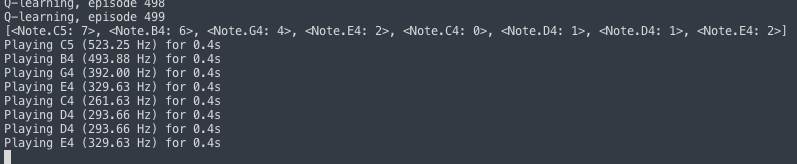
\includegraphics[width=\linewidth]{it500.jpg}
  \caption{Iteration 500: Not efficient policy due to note transitions like C4 to D4 in position 5}
  \label{fig:it500}
\end{figure}

As we can see in Figure \ref{fig:it500}, the optimal policy was not found yet, since the algorithm is still deciding to use a higher note in the position 6 than the previous note (position 5).

\begin{figure}[ht]
  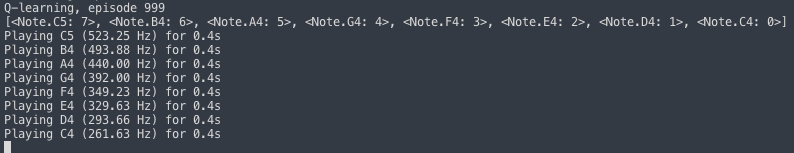
\includegraphics[width=\linewidth]{it1000.png}
  \caption{Iteration 1000: Optimal policy. Each note is lower than the previous one.}
  \label{fig:it1000}
\end{figure}

\newpage

In Figure \ref{fig:it1000} we notice that the algorithm finally found the optimal policy for the scenario that we proposed (each note should be lower than the previous one). Of course, this condition does not have any musical validity, it was only used for testing the learning capability of our algorithm.



\section*{Conclusion}
We are expecting to complete the following changes in the future releases in order to improve our results:

\begin{itemize}
  \item 11/8: Persist the \emph{(state, action)} values for future training. The matrix of values could be stored in a file for continuing the training later.
  \item 11/15: Enable different durations for notes. We plan to include the duration of the note in the state.
  \item 11/25: Finish project presentation and report.
  \item Desirable: Start using relative values instead of the notes itself. We need to modify the values for our notes in our state based on a melodies tonality. The tonality initially will be an hyperparameter in our algorithm.
  \item Desirable: Include \emph{chords} in the composition process. This will enable us to translate the notes based on the chord and not in the tonality hyperparameter. We are planning to include the chord as part of the state.
  \item Desirable: Include Neural Network with our q-learning learning algorithm. The approach will follow the process from the assignments using PyTorch.
  \item Desirable: Start using RNN and Monte Carlo for the learning process. More research will be necessary in order to determine the effort needed for this task.
\end{itemize}

Based on the progress done so far, we have been able to adapt the musical composition problem to a Reinforcement Learning scenario. We were able to use \emph{q-learning} in order to learn \emph{musical policies} that allow us to know which note should follow a previous sequence of notes. We were able to test how our algorithm learn based on the input provided by the user, and we included an automated test in order to verify that the algorithm was adequately learning the appropriate values for each \emph{(state, action)}. Finally, we detailed the future enhancements that we are planing to include for the future releases of our project with its respective methodology and that way improve the results that we are getting in order to get more pleasant melodies.

\bibliographystyle{unsrtnat}
\bibliography{fvilchez}

\end{document}